%! TEX root = main.tex

\graphicspath{{00_Images/08_chapter/}}

\chapter{Circuit Analysis: the Tube Screamer}
\label{ch:tubescreamer}

\section{General Overview}
\label{sc:81}

The Ibanez Tube Screamer is one of the most widely used overdrive pedals in electric guitar history, and its circuit gathers in a single compact unit nearly every building block introduced in the preceding chapters: a discrete transistor buffer, a non-inverting operational amplifier stage, a non-linear clipping network, and a passive-active tone-shaping filter.
For this reason it serves as an ideal case study, in the same spirit as the MXR Distortion+ analyzed in chapter \ref{ch:mxr}, but with a more sophisticated distortion mechanism and an explicit tone control.
The defining sonic feature of the Tube Screamer is that it emulates the gradual saturation of a thermionic valve amplifier rather than the abrupt limiting of a solid-state clipper, which is the origin of its name.

\begin{figure}[!htb]
    \centering
    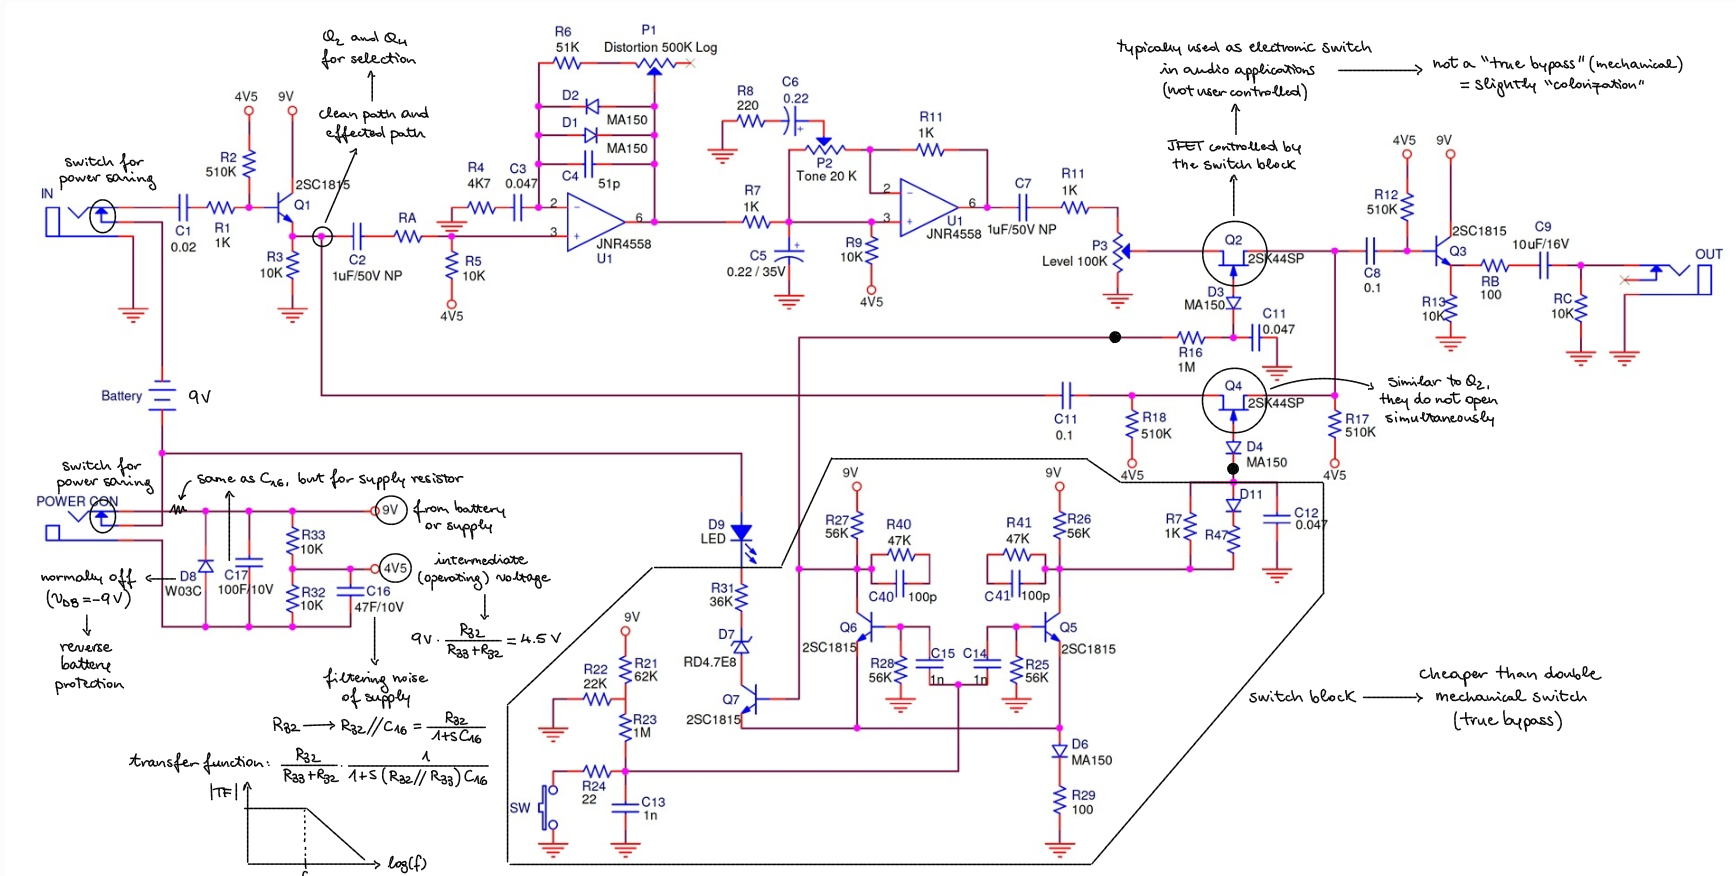
\includegraphics[width=0.8\textwidth]{Tube_Screamer_Full.png}
    \caption{Complete schematic of the Tube Screamer overdrive pedal}
    \label{fig:tsFull}
\end{figure}

The complete schematic of figure \ref{fig:tsFull} contains the power supply network, the true-bypass switching, and the effect path itself.
Only the effect path is relevant to the signal-processing analysis, and it can be decomposed into four cascaded modules, each treated separately in the sections that follow.
The four modules of figure \ref{fig:tsEffectPath} are the input buffer, realized as a common-collector stage that isolates the high-impedance guitar pickup from the rest of the circuit; the distortion block, a non-inverting operational amplifier with diodes placed in the feedback loop; the tone control, an active shelving filter built around the potentiometer \(P_2\); and the output stage, comprising a level-control fader and an output buffer.
The supply rail of the pedal is a single \SI{9}{\volt} battery, so all the active stages are biased around a mid-supply reference of \SI{4.5}{\volt}, exactly as discussed for the MXR Distortion+ in chapter \ref{ch:mxr}, allowing the AC signal to swing symmetrically about the quiescent point without a negative supply.

\begin{figure}[!htb]
    \centering
    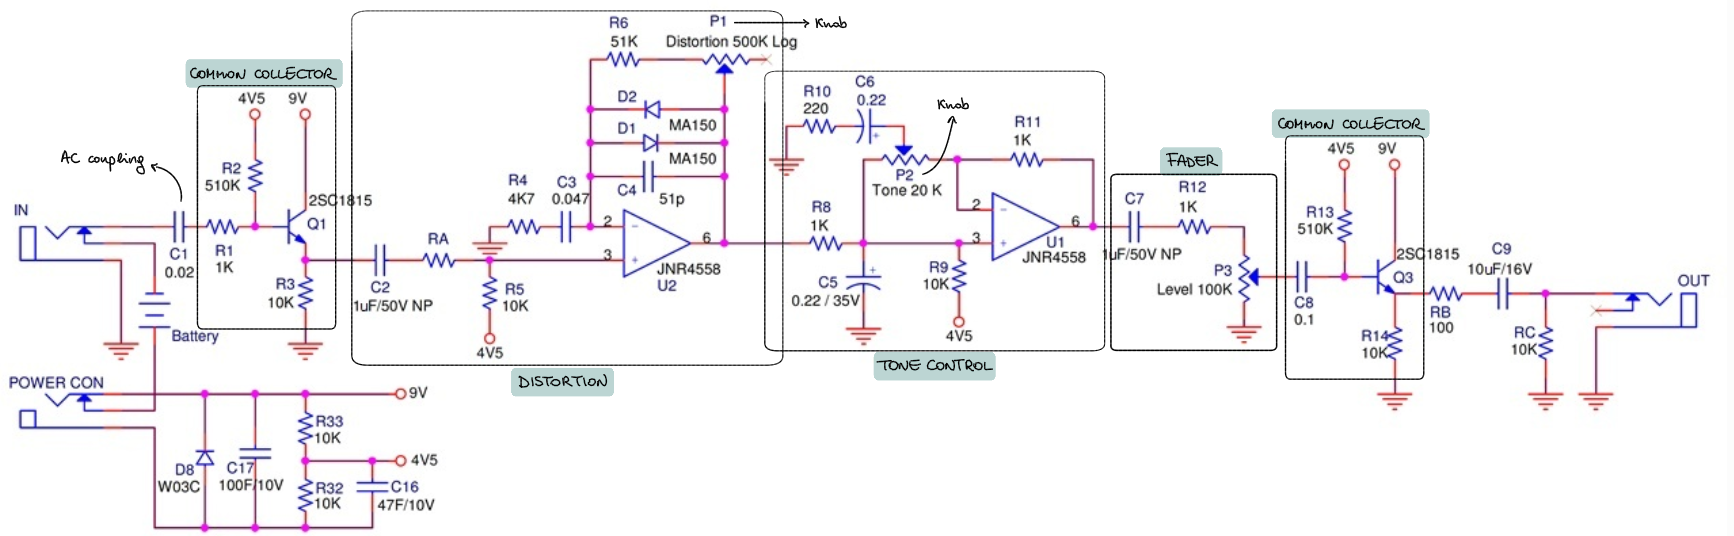
\includegraphics[width=0.80\textwidth]{Tube_Screamer_Effect_Path.png}
    \caption{Decomposition of the effect path into its four functional modules: input buffer, distortion block, tone control, and output level control}
    \label{fig:tsEffectPath}
\end{figure}

\section{DC and AC Analysis of the Input Buffer}
\label{sc:82}

The first module is a common-collector stage, also called an emitter follower, whose function is to present a very high input impedance to the guitar pickup and a very low output impedance to the following stage, transferring the signal without loading the source.

\begin{figure}[!htb]
    \centering
    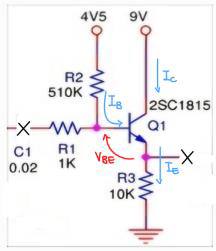
\includegraphics[width=0.40\textwidth]{Tube_Screamer_Common_Collector_1.png}
    \caption{Input buffer of the Tube Screamer: a common-collector stage biased from the mid-supply rail through \(R_2\), with the emitter resistor \(R_3\) setting the operating current}
    \label{fig:tsCC1}
\end{figure}

\subsection{DC Bias Point}
\label{ssc:821}

In the DC analysis all the coupling capacitors behave as open circuits, so the bias network reduces to the base resistor \(R_2\) connected to the mid-supply rail and the emitter resistor \(R_3\) to ground.
The base current is set by the voltage drop across \(R_2\):
\[
I_B = \frac{\SI{4.5}{\volt} - V_B}{R_2}
\]
Adopting the standard active-region hypothesis \(V_{BE} \approx \SI{0.7}{\volt}\), the emitter voltage follows the base voltage, and the emitter current is
\[
I_E = (\beta + 1) I_B = \frac{V_E}{R_3} = \frac{V_B - \SI{0.7}{\volt}}{R_3}
\]
Solving for the base voltage gives \(V_B = \SI{0.7}{\volt} + R_3(\beta + 1)I_B\), and substituting the expression for \(I_B\) couples the two relations into a single equation in \(V_B\):
\[
V_B\left(1 + \frac{R_3}{R_2}(\beta + 1)\right) = \SI{0.7}{\volt} + \frac{R_3}{R_2}(\beta + 1)\cdot\SI{4.5}{\volt}
\]
from which the bias voltage is obtained in closed form:
\[
V_B = \frac{\SI{0.7}{\volt} + \dfrac{R_3}{R_2}(\beta + 1)\cdot\SI{4.5}{\volt}}{1 + \dfrac{R_3}{R_2}(\beta + 1)}
\]

With the component values \(R_2 = \SI{510}{\kilo\ohm}\), \(R_3 = \SI{10}{\kilo\ohm}\), so that \(R_3/R_2 = 1/51\), and a typical current gain \(\beta = 300\), the base settles at \(V_B \approx \SI{3.94}{\volt} \approx \SI{4}{\volt}\).
The emitter then sits at \(V_E = V_B - V_{BE} = \SI{3.3}{\volt}\), and since \(I_C \approx I_E = V_E/R_3\), the quiescent collector current is
\[
I_C \approx \SI{330}{\micro\ampere}, \qquad I_B = \frac{I_C}{\beta} = \SI{1.1}{\micro\ampere}
\]
These bias values fix the small-signal parameters of the device, the transconductance and the base-emitter resistance:
\[
g_m = \frac{I_C}{V_T} = \frac{\SI{330}{\micro\ampere}}{\SI{26}{\milli\volt}} \approx \SI{13.2}{\milli\siemens}, \qquad r_\pi = \frac{\beta}{g_m} = \frac{\beta V_T}{I_C} \approx \SI{22}{\kilo\ohm}
\]

\subsection{Small-Signal Behavior and AC Coupling}
\label{ssc:822}

The small-signal analysis of this stage is identical to the emitter follower derived in detail in section \ref{sc:74}, where the supply rail acts as an AC ground and the BJT is replaced by its hybrid-\(\pi\) model.
The same derivation yields an input impedance \(Z_{in} = r_\pi + (\beta + 1)R_3 = \SI{22}{\kilo\ohm} + 301\times\SI{10}{\kilo\ohm} \approx \SI{3}{\mega\ohm}\), a near-unity voltage gain
\[
\frac{v_{out,CC}}{v_{in,CC}} = \frac{g_m R_3}{1 + g_m R_3} \approx 1 \qquad \text{since } g_m R_3 \gg 1
\]
and a very low output impedance of the order of \(1/g_m\).
The stage therefore performs no voltage amplification, but transforms the impedance level: it accepts the weak, high-impedance pickup signal without attenuating it and drives the subsequent distortion block from a stiff, low-impedance source.

The buffer is coupled to the source and to the following stage through series capacitors, which together with the bias resistors form a high-pass network.
This AC coupling blocks the DC bias component, so that only the signal is passed forward, and it sets the lower edge of the audio passband below which the gain rolls off, as shown by the transfer function of figure \ref{fig:tsACcoupling}.

\begin{figure}[!htb]
    \centering
    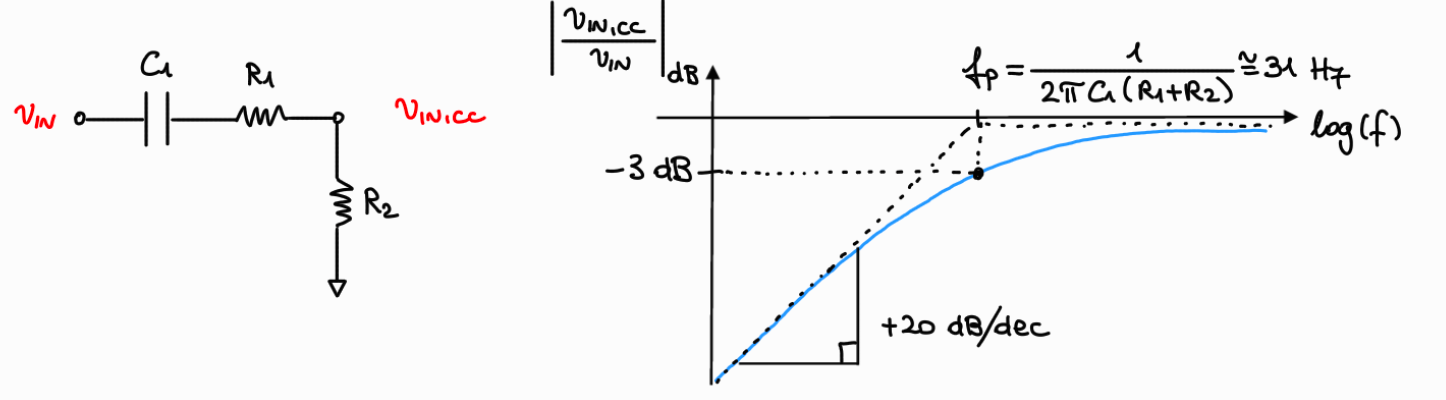
\includegraphics[width=0.65\textwidth]{Tube_Screamer_Common_Collector_1_filter.png}
    \caption{High-pass transfer function introduced by the input AC-coupling capacitors, which decouple the DC bias and set the low-frequency limit of the buffer}
    \label{fig:tsACcoupling}
\end{figure}

\section{The Distortion Block}
\label{sc:83}

The distortion block is the heart of the pedal, where the controlled non-linearity responsible for the overdrive timbre is generated.
It is built as a non-inverting operational amplifier whose feedback network contains a pair of anti-parallel diodes, and its analysis proceeds in two steps: first the linear response with the diodes removed, then the non-linear clipping behavior they introduce.

\begin{figure}[!htb]
    \centering
    \subfloat[Full schematic of the distortion block]{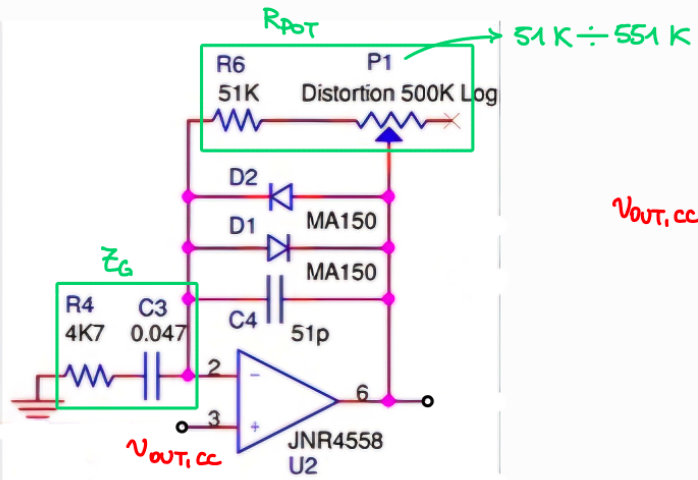
\includegraphics[height=0.22\textheight]{Tube_Screamer_Distorsion_Block_Full.png}}
    \hfill
    \subfloat[Generalized non-inverting stage with input impedance \(Z_G\) and feedback impedance \(Z_F\)]{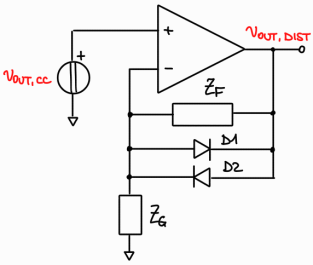
\includegraphics[height=0.22\textheight]{Tube_Screamer_Distorsion_Block.png}}
    \caption{The distortion block as a non-inverting amplifier: complete schematic and its generalized impedance representation}
    \label{fig:tsDistBlock}
\end{figure}

\subsection{Linear Response}
\label{ssc:831}

Neglecting the diodes, the block is a non-inverting amplifier whose gain is set by the ratio of a feedback impedance \(Z_F\) to a grounded input impedance \(Z_G\), as represented in figure \ref{fig:tsDistBlock}.
The input branch is a resistor in series with a capacitor, while the feedback branch is the tone-and-gain potentiometer in parallel with a small capacitor:
\[
Z_G = R_4 + \frac{1}{sC_3} = \frac{1 + sC_3 R_4}{sC_3}, \qquad Z_F = R_{POT} || \frac{1}{sC_4} = \frac{R_{POT}}{1 + sC_4 R_{POT}}
\]
where \(R_{POT} = R_6 + P_1\) is the series combination of a fixed resistor and the drive potentiometer, adjustable over the range \(R_{POT} \in [\SI{51}{\kilo\ohm}, \SI{551}{\kilo\ohm}]\).
The non-inverting transfer function is therefore
\[
\frac{v_{out,DIST}}{v_{out,CC}} = 1 + \frac{Z_F}{Z_G} = 1 + \frac{R_{POT}}{1 + sC_4 R_{POT}} \cdot \frac{sC_3}{1 + sC_3 R_4}
\]

The exact expression carries the additive unity term, which must be retained in any rigorous calculation.
A simplified form is sometimes used to read off the pole and zero structure, but it is only an approximation and discards the unity term:
\[
\frac{v_{out,DIST}}{v_{out,CC}} \approx \frac{R_{POT}}{1 + sC_4 R_{POT}} \cdot \frac{sC_3}{1 + sC_3 R_4}
\]
In this approximate form the response has one zero at the origin and two poles, with corner frequencies
\[
f_{p1} = \frac{1}{2\pi R_4 C_3} = \SI{720}{\hertz}, \qquad f_{p2} = \frac{1}{2\pi R_{POT} C_4}
\]
where \(C_3 = \SI{0.047}{\micro\farad}\) and \(R_4 = \SI{4.7}{\kilo\ohm}\) fix the first pole, while the second pole moves with the drive setting over the range \(f_{p2} \in [\SI{5.7}{\kilo\hertz}, \SI{61}{\kilo\hertz}]\), the lower edge corresponding to maximum \(R_{POT}\) and the upper edge to minimum \(R_{POT}\).

\begin{figure}[!htb]
    \centering
    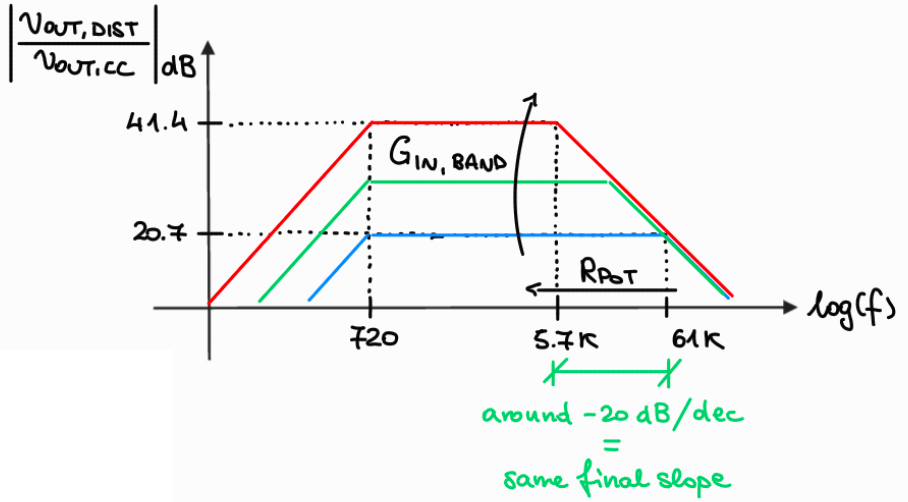
\includegraphics[width=0.70\textwidth]{Distorsion_Block_Transfer_Function.png}
    \caption{Magnitude response of the distortion block: a band-pass shape with a flat mid-band region whose gain is set by the drive control}
    \label{fig:tsDistTF}
\end{figure}

In the mid-band region \(f \in [f_{p1}, f_{p2}]\), the capacitor \(C_3\) behaves as a short circuit and \(C_4\) as an open circuit, so the gain flattens to the resistive ratio
\[
G_{in,band} = \frac{R_{POT}}{R_4} \in [10.8, 117.2] \equiv [\SI{20.7}{\decibel}, \SI{41.4}{\decibel}]
\]
The drive control thus sweeps the mid-band gain over more than \SI{20}{\decibel}, directly setting how hard the signal is pushed into the clipping region described next.

\subsection{Non-Linear Clipping Behavior}
\label{ssc:832}

The anti-parallel diodes in the feedback path remain inactive as long as the voltage across them is below the forward threshold of \SI{0.7}{\volt}.
Since the inverting input is a virtual copy of the buffered input, the diode stays off while \(v_{out} - v^{-} < \SI{0.7}{\volt}\), which using the mid-band gain becomes
\[
\frac{R_{POT}}{R_4} v_{in} < \SI{0.7}{\volt} \quad \Rightarrow \quad v_{in} < \SI{0.7}{\volt}\cdot\frac{R_4}{R_{POT}} = \frac{\SI{0.7}{\volt}}{G_{in,band}}
\]
For the representative setting \(G_{in,band} = 10\), the diodes begin to conduct when the input reaches \(v_{in} = \SI{70}{\milli\volt}\), at which point the output has grown to \(v_{out} = \SI{770}{\milli\volt}\).

\begin{figure}[!htb]
    \centering
    \subfloat[Distortion block with the feedback diodes and the resulting clamped output]{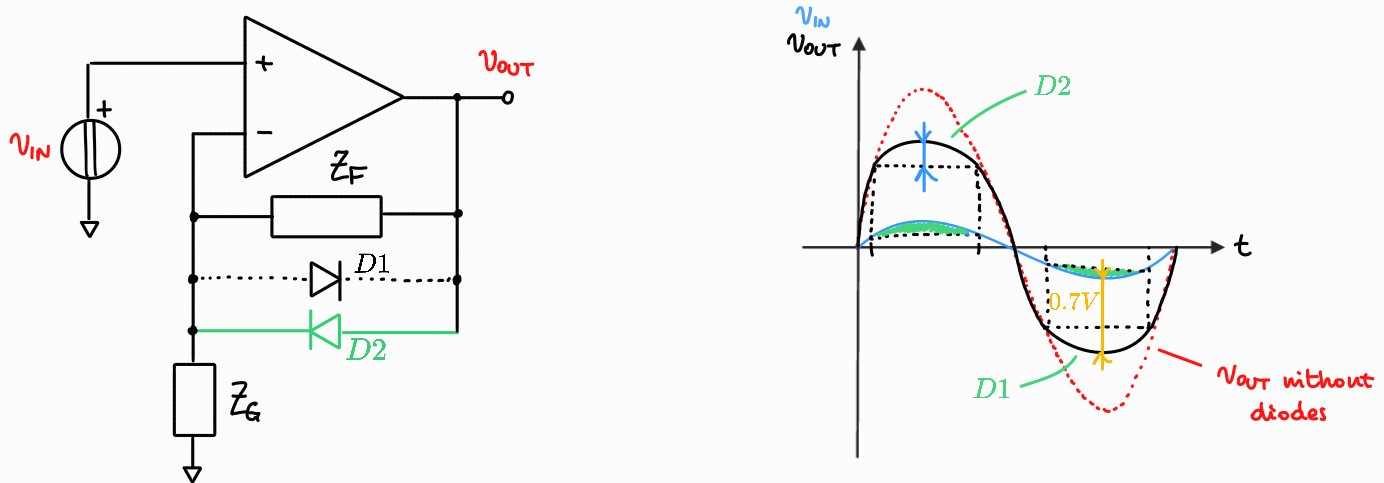
\includegraphics[width=0.70\textwidth]{Distortion_Block_Diodes.png}}
    \\
    \subfloat[Soft clipping versus hard clipping of the output waveform]{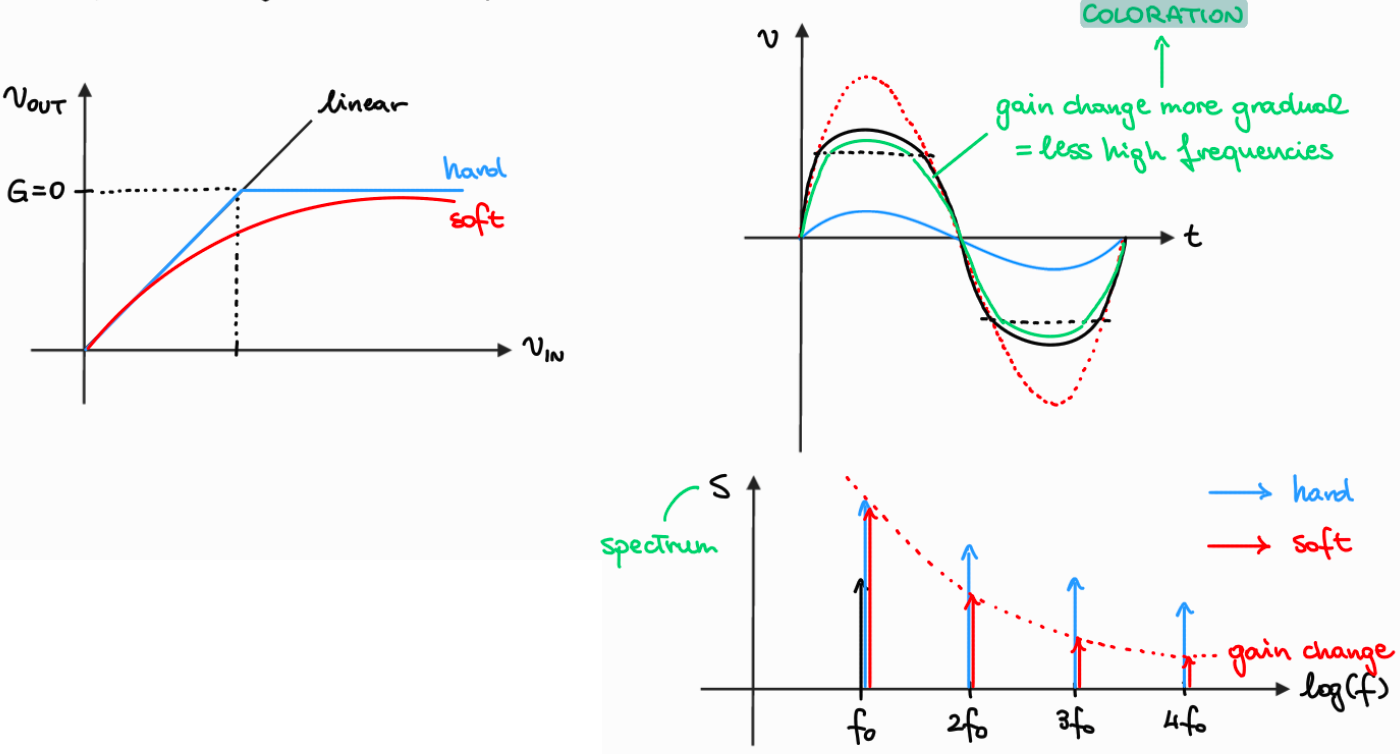
\includegraphics[width=0.70\textwidth]{Soft_Hard_Clipping.png}}
    \caption{Clipping mechanism of the Tube Screamer: once a diode conducts it behaves as a \SI{0.7}{\volt} source in the feedback loop, rounding the waveform smoothly rather than truncating it}
    \label{fig:tsSoftClip}
\end{figure}

The crucial difference with the MXR Distortion+ of section \ref{sc:34} lies in where the diodes are connected.
In the MXR the diodes are placed from the output node to ground, so once they conduct they clamp the output hard at \SI{0.7}{\volt} and the gain collapses abruptly toward zero, truncating the waveform: this is hard clipping.
In the Tube Screamer the diodes sit inside the feedback loop, so when one of them conducts it behaves as a \SI{0.7}{\volt} source that lowers the effective feedback impedance, driving the closed-loop gain asymptotically toward unity rather than to zero.
The output then continues to track the input with unity incremental gain instead of being flattened, producing the gentle, rounded saturation known as soft clipping, illustrated in figure \ref{fig:tsSoftClip}.
This progressive reduction of gain, rather than an abrupt cut, is precisely the behavior of an overdriven valve stage, and it is the reason the pedal is perceived as warm and tube-like.
Because the gain decreases gradually as the signal grows, the amount of soft clipping increases smoothly with drive, generating a rich set of harmonics whose spectral content varies with the playing level, the so-called coloration of the sound.

\section{Tone Control}
\label{sc:84}

The final processing module is the tone control, an active shelving filter that shapes the harmonic content generated by the distortion block.
Its purpose is to attenuate the high-frequency harmonics produced by the saturation, softening the harshness of the spurious components, in the same family of shelving circuits analyzed for equalizers in section \ref{sc:532}.

\begin{figure}[!htb]
    \centering
    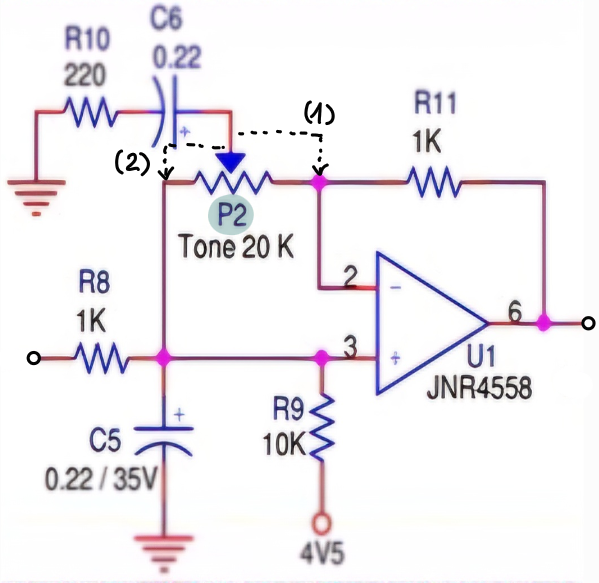
\includegraphics[width=0.45\textwidth]{Tube_Screamer_Tone_Control.png}
    \caption{Tone control module: the potentiometer \(P_2\) selects how the shaping network is connected to the operational amplifier}
    \label{fig:tsTone}
\end{figure}

The behavior of the module of figure \ref{fig:tsTone} is governed by the position of the potentiometer \(P_2\), which switches the connection of the shaping network between the inverting input, denoted configuration 1, and the non-inverting input, denoted configuration 2.
The two extreme positions define the limits of the tonal sweep, and intermediate settings interpolate smoothly between them.

\subsection{Configuration 1}
\label{ssc:841}

In the first configuration the network is referred to the inverting input, and the voltage reaching the non-inverting terminal is set by the divider formed by \(R_8\) and the parallel combination of \(R_9\) with the capacitor \(C_5\):
\[
v^{+} = \frac{R_9 || Z_{C5}}{R_8 + R_9 || Z_{C5}} v_{in}, \qquad Z_{C5} = \frac{1}{sC_5}
\]

\begin{figure}[!htb]
    \centering
    \subfloat[Tone network referred to the inverting input]{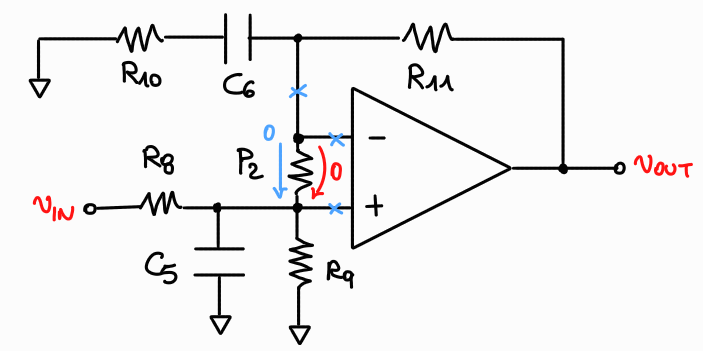
\includegraphics[height=0.14\textheight]{Tube_Screamer_Tone_Control_Config_1.png}}
    \hfill
    \subfloat[Reduced network used to evaluate \(v^{+}\)]{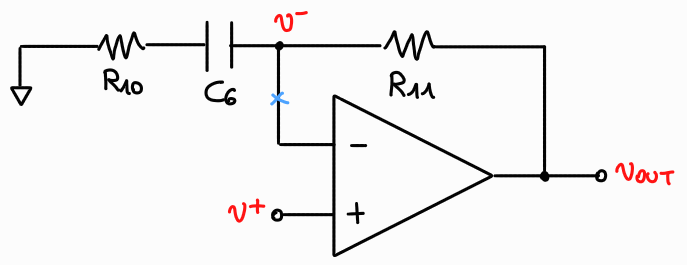
\includegraphics[height=0.14\textheight]{Tone_Control_Config_1_continued.png}}
    \caption{Configuration 1 of the tone control and the simplified network for the transfer-function derivation}
    \label{fig:tsToneCfg1}
\end{figure}

Collecting the divider into a low-frequency gain term multiplied by a single pole, and recognizing the parallel resistance \(R_8 || R_9\), the transfer function takes the compact shelving form
\[
\frac{v^{+}}{v_{in}} = \frac{R_9}{R_8 + R_9}\cdot\frac{1}{1 + sC_5(R_8 || R_9)}
\]
The operational amplifier then applies the feedback network around \(R_{10}\), \(R_{11}\), and \(C_6\), contributing a second shelving factor:
\[
\frac{v_{out}}{v^{+}} = 1 + \frac{R_{11}}{R_{10} + \dfrac{1}{sC_6}} = \frac{1 + sC_6(R_{10} + R_{11})}{1 + sC_6 R_{10}}
\]
The overall response is the product of the two factors: a passive high-cut shelf followed by an active shelf, whose combined effect is shown in figure \ref{fig:tsToneTF1}.

\begin{figure}[!htb]
    \centering
    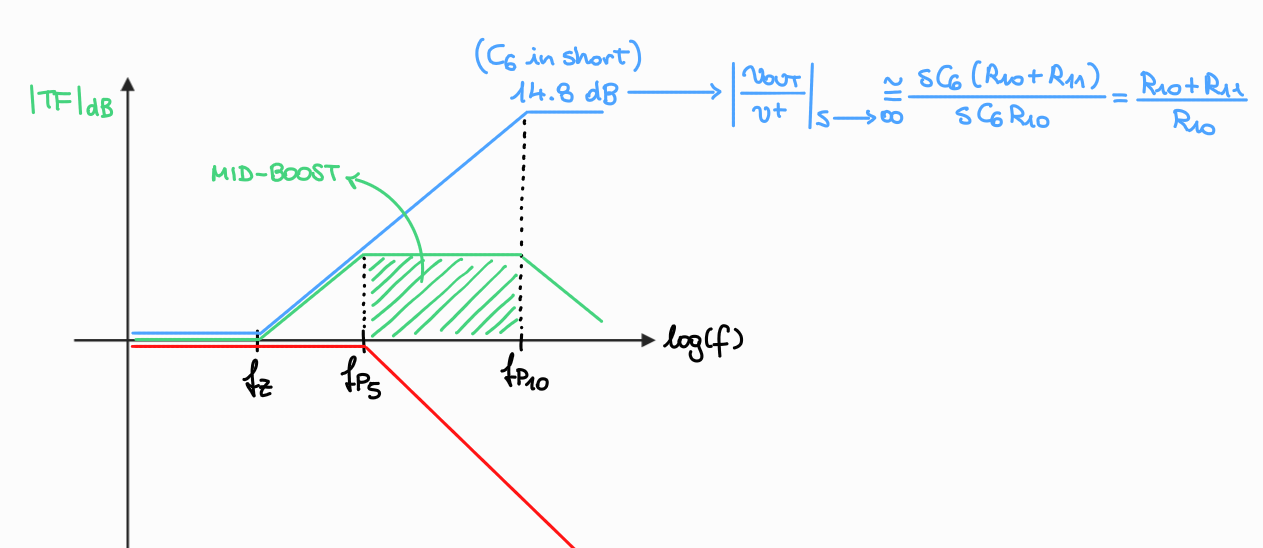
\includegraphics[width=0.70\textwidth]{Tube_Screamer_Tone_Control_Graph.png}
    \caption{Magnitude response of the tone control in configuration 1, showing the high-frequency attenuation that smooths the saturation harmonics}
    \label{fig:tsToneTF1}
\end{figure}

\subsection{Configuration 2}
\label{ssc:842}

In the second configuration the shaping network is referred to the non-inverting input, and it is convenient to lump the whole branch into a single equivalent impedance:
\[
Z_{eq} = R_9 || Z_{C5} || \left(R_{10} + \frac{1}{sC_6}\right)
\]

\begin{figure}[!htb]
    \centering
    \subfloat[Tone network referred to the non-inverting input]{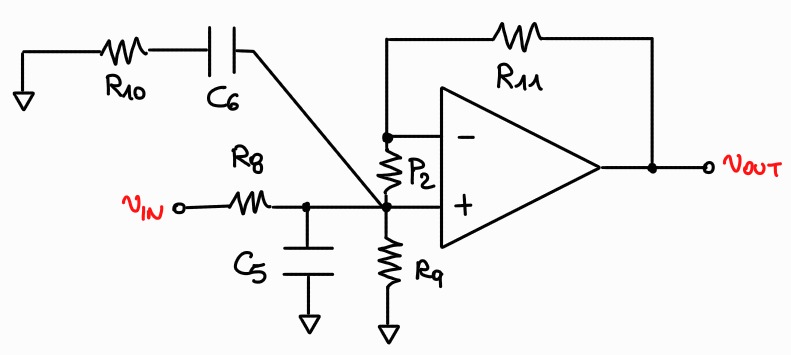
\includegraphics[height=0.16\textheight]{Tube_Screamer_Tone_Control_Config_2.png}}
    \hfill
    \subfloat[Representation through the equivalent impedance \(Z_{eq}\)]{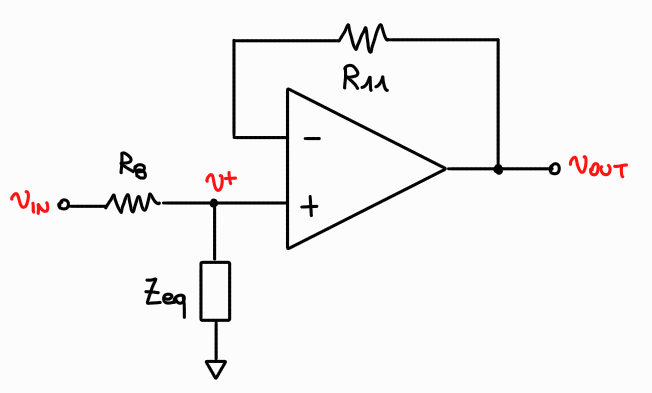
\includegraphics[height=0.16\textheight]{Tube_Screamer_Tone_Control_Config_2_2.png}}
    \caption{Configuration 2 of the tone control and its reduction to a single equivalent impedance}
    \label{fig:tsToneCfg2}
\end{figure}

The voltage at the non-inverting input is then a divider between \(R_8\) and \(Z_{eq}\), and after expansion the response factors into one zero and two poles:
\[
\frac{v^{+}}{v_{in}} = \frac{Z_{eq}}{Z_{eq} + R_8} = \frac{1 + sT_2}{(1 + sT_{p1})(1 + sT_{p2})}
\]
The resulting transfer function sits between the two extremes, so that rotating \(P_2\) from configuration 1 toward configuration 2 slides the high-cut corner continuously, brightening or darkening the tone.
The two limiting responses and the family of intermediate curves are shown in figure \ref{fig:tsToneTF2}.

\begin{figure}[!htb]
    \centering
    \subfloat[Magnitude response in configuration 2]{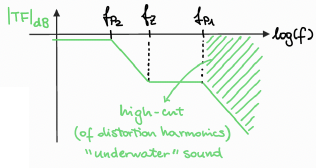
\includegraphics[height=0.20\textheight]{Tone_Control_2_Transfer_Function.png}}
    \\
    \subfloat[Variation of the response between the full-left and full-right settings]{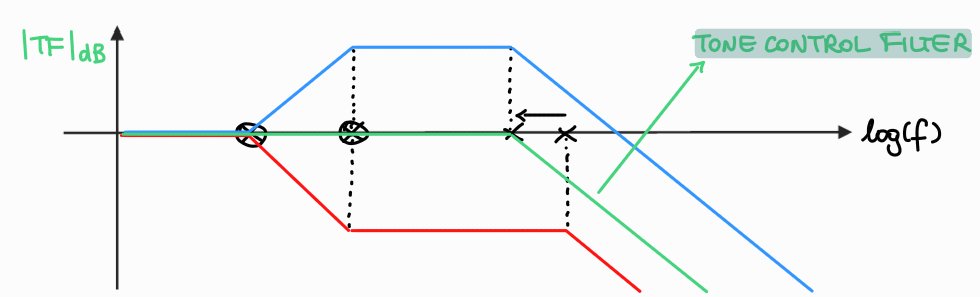
\includegraphics[width=0.80\textwidth]{Tone_Control_Final_TF.png}}
    \caption{Tone-control response in configuration 2 and the continuous variation obtained as the potentiometer sweeps between its two extremes}
    \label{fig:tsToneTF2}
\end{figure}

The tone control therefore acts as a variable high-cut filter applied after the non-linear stage, attenuating the upper harmonics generated by the saturation to a degree chosen by the player.
This high-frequency shaping is the second mechanism, alongside the soft clipping itself, by which the Tube Screamer imparts its characteristic smooth and warm coloration.
